\documentclass[a4paper, 12pt]{article}

\usepackage[T2A]{fontenc}
\usepackage[utf8]{inputenc}
\usepackage[english,russian]{babel}
\usepackage[left=15mm, top=20mm, right=15mm, bottom=20mm, nohead, nofoot]{geometry}

\usepackage{graphicx}
\graphicspath{{pictures/}}
\DeclareGraphicsExtensions{.pdf,.png,.jpg}
\usepackage{multirow}
\usepackage{wrapfig}
\usepackage{afterpage}
\usepackage{amsmath, amsfonts, amssymb, amsthm, mathtools}
\author{Маллаев Руслан, группа Б02-005}
\title{Лабораторная работа № 1.2.5 \\ Гироскоп
}
\date{9 ноября 2020 г.}

\begin{document}

\maketitle
\thispagestyle{empty}
\newpage
\textbf{Цель работы:} Исследовать вынужденную прецессию гироскопа и определить скорость вра-

щения ротора гироскопа и сравнить ее со скоростью, рассчитанной по скорости прецессии.\\

\textbf{Приборы, используемые в работе:} гироскоп в кардановом подвесе, секундомер, набор

грузов, отдельный ротор гироскопа, цилиндр известной массы, крутильный маятник, штан-

генциркуль, линейка.\\

Соберем установку, как показано на рисунке 1:
\[\text{Рисунок №1}\]
\begin{center}
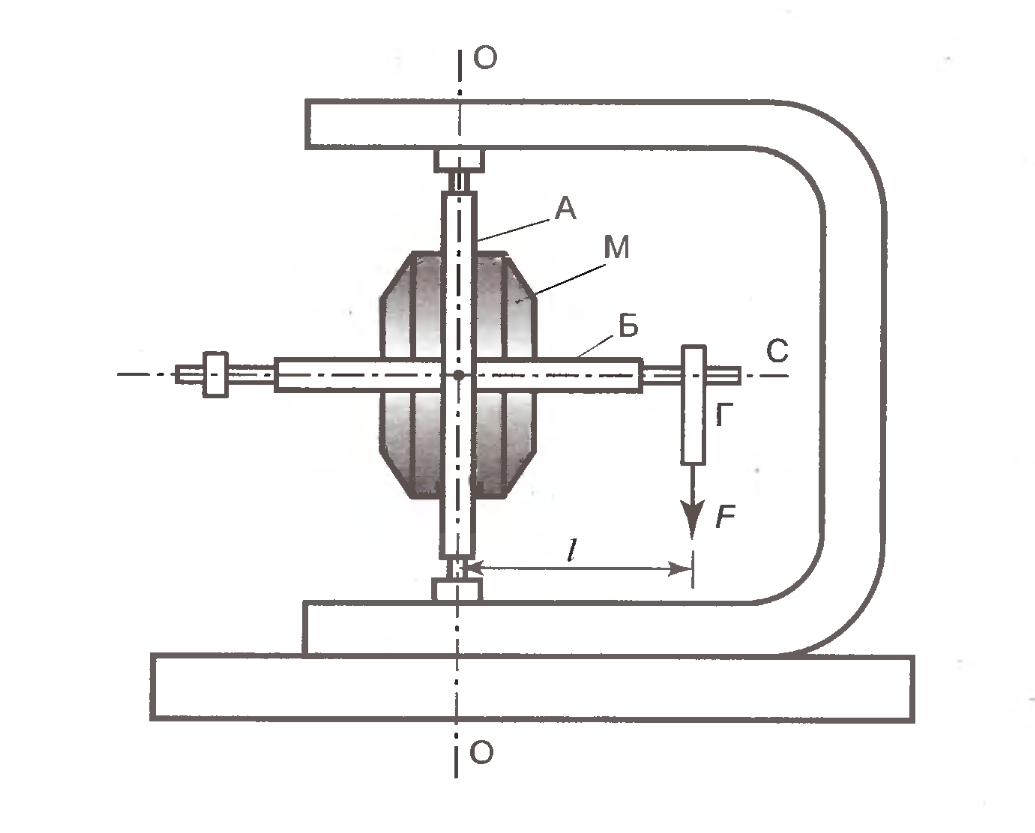
\includegraphics[scale=0.6]{giro}
\end{center}

\newpage
\section{Настройка гироскопа}

Устанавливаем ось гироскопа в горизонтальное положение и включаем его на 5 минут, чтобы стабилизировалось вращение ротора.

При нажатии на рычаг гироскоп вращается по часовой стрелке, если смотреть сверху. Из этого можно сделать вывод, что ротор вращается по часовой стрелке, если смотреть со стороны гайки.

Длина рычага $l = 120 \text{мм}$

\section{Измерение угловой скорости регулярной прецессии $\Omega$}

$T_i$ - i-ое измерение времени одного оборота гироскопа(так как при большем количестве оборотов рычаг опускается слишком сильно); $h_0 \text{ и }h_{\text{к}}$ - высота края рычага над столом до поворота и после, соответственно.

\begin{center}
\begin{tabular}{|c|c|c|c|c|c|c|c|c|c|c|c|}
\hline
m, г   & $T_1$, c  & $T_2$, c  & $h_{01}$, см  & $h_{02}$, см  & T, c     & $\Omega$, $c^{-1}$  & $h_{\text{к}1}$, см  & $h_{\text{к}2}$, см  & $\upsilon_1$, м/с     & $\upsilon_2$, м/с     & $\upsilon$, м/с       \\ \hline
61  & 163 & 162 & 17.0 & 17.5 & 163 & 0.039 & 14.7 & 15.0 & 0.014 & 0.015 & 0.015 \\ \hline
77  & 131 & 131 & 16.9 & 16.2 & 131 & 0.048 & 14.9 & 14.2 & 0.015 & 0.015 & 0.015 \\ \hline
93  & 107 & 108 & 16.7 & 16.1 & 108 & 0.058 & 14.9 & 14.4 & 0.017 & 0.016 & 0.016 \\ \hline
142 & 70  & 71  & 17.0 & 16.0 & 71  & 0.089 & 15.9 & 15.1 & 0.016 & 0.013 & 0.014 \\ \hline
214 & 46  & 46  & 17.0 & 16.5 & 46  & 0.137  & 16.0 & 15.7 & 0.022 & 0.017 & 0.020\\ \hline
335 & 29  & 29  & 17.0 & 16.2 & 29  & 0.217  & 16.2 & 15.7 & 0.028 & 0.017 & 0.022\\ \hline
\end{tabular}
\end{center}
\[T = \frac{T_1 + T_2}{2}\]
\[\upsilon_i = \frac{h_{0i} - h_{\text{к}i}}{T}\]
\[\upsilon = \frac{\upsilon_1 + \upsilon_2}{2}\]
\[\Omega = \frac{2\pi}{T}\]
\[M = m\cdot g\cdot\l\]
\begin{center}
\begin{tabular}{|c|c|c|}
\hline
m, г   & $\Omega$, $c^{-1}$  & M, Н$\cdot$м     \\ \hline
61  & 0.039 & 0.072 \\ \hline
77  & 0.048 & 0.091 \\ \hline
93  & 0.058 & 0.109 \\ \hline
142 & 0.089 & 0.167 \\ \hline
214 & 0.137  & 0.252 \\ \hline
335 & 0.217  & 0.394 \\ \hline
\end{tabular}
\end{center}

\[\Omega = \frac{M}{I_z\cdot\omega_0}\]
Построим график зависимости $\Omega$ от M на графике №1:
\begin{center}
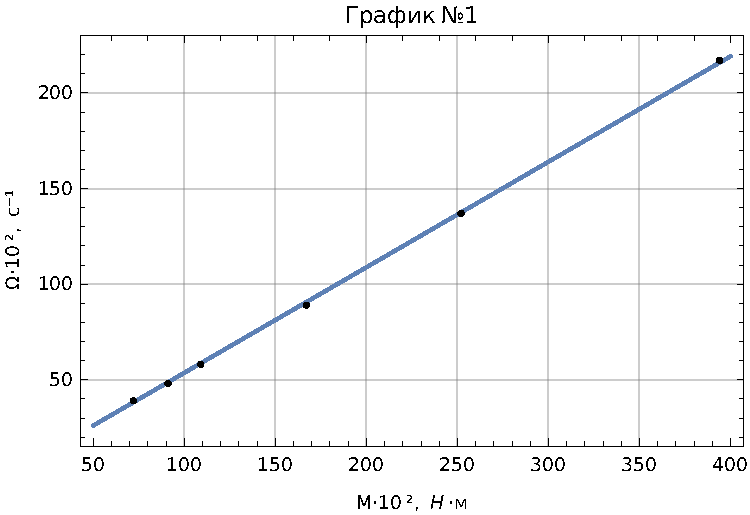
\includegraphics[scale=1]{omeM}
\end{center}
Отсюда получаем коэффициент наклона графика функции:
\[k = 0.551474\frac{1}{H\cdot\text{м}\cdot c}\]

\section{Измерение момента инерции ротора}
Дважды измерим время десяти крутильных колебаний ротора и усредним полученное значение:
\[T_{p10} = \frac{31.66 + 31.88}{2} c = 31.77 c\]
то есть период крутильного колебания ротора:
\[T_0 = \frac{T_{p10}}{10} = 3.18c\]
Дважды измерим время десяти крутильных колебаний цилиндра известной массы $m_{\text{ц}} = 1617.8$ г и известного радиуса $R_{\text{ц}} = 3.92$ см и поделим на 10 усредненное значение, чтобы найти период крутильных колебаний данного цилиндра:
\[T_{\text{ц}} = \frac{39.87 + 39.94}{20}c = 3.99c\]
\[I_{\text{ц}} = \frac{m_{\text{ц}}\cdot R^2_{\text{ц}}}{2} = 12.4\cdot10^{-4}\text{кг}\cdot\text{м}^2\]
Тогда, по формуле:
\[I_0 = I_{\text{ц}}\cdot\frac{T_0^2}{T_{\text{ц}}^2} = 7.9\cdot10^{-4}\text{кг}\cdot\text{м}^2\]
\newpage
\section{Расчет частоты вращения ротора гироскопа}
\[k = \frac{1}{I_0\cdot\omega_0}\]
Тогда:
\[\frac{\omega_0}{2\pi} = f = \frac{1}{k\cdot I_0} = 365.6 \text{Гц}\]
\[\sigma_{I_0} = I_0\sqrt{2(\frac{\sigma_{T_{\text{ц}}}}{T_{\text{ц}}})^2 + 2(\frac{\sigma_{T_0}}{T_0})^2 + (\frac{\sigma_{I_{\text{ц}}}}{I_{\text{ц}}})^2}\]
Откуда:
\[f = 366 \pm 8 \text{ Гц} \]
\section{Измерение частоты вращения ротора при помощи фигур Лиссажу}
Выключу гироскоп и начну изменять частоту на генераторе, пока на экране осциллографа не появится фигура Лиссажу. Сниму зависимость частоты ротора от времени:
\begin{center}
\begin{tabular}{|c|c|c|c|c|c|c|c|c|c|c|c|c|c|c|}
\hline
$f$, Гц & 384 & 377 & 373 & 370 & 367 & 362 & 359 & 356 & 354 & 347 & 330 & 320 & 310 & 300 \\ \hline
$t$, с & 17  & 38  & 49  & 58  & 67  & 82  & 93  & 101 & 107 & 129 & 184 & 217 & 250 & 285 \\ \hline
\end{tabular}
\end{center}
 Построим график зависимости $f$ от $t$ и найдем свободный член зависимости, чтобы определить $f(0)$:
\begin{center}
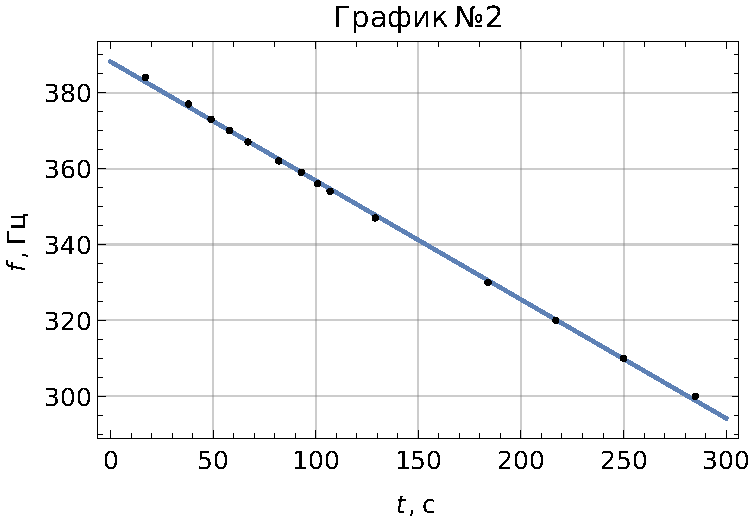
\includegraphics[scale=1]{freqt}
\end{center}
$f = 388.17 \pm 2.11$ Гц из графика



\end{document}
